\documentclass[tikz, border = 1 cm]{standalone}

%%%%%%%%%%%%%%
\usepackage{tikz}
\usetikzlibrary{decorations, decorations.markings, arrows, positioning}
%%%%%%%%%%%%%%

%%%%%%%%%%%%%%
\definecolor{blue1}{RGB}{0,177,234}
\definecolor{blue4}{RGB}{178,231,248}
\definecolor{gray1}{RGB}{76,84,93}
\definecolor{gray4}{RGB}{201,203,206}
\definecolor{bluegray1}{RGB}{0,127,167}
\definecolor{bluegray4}{RGB}{178,216,228}
\definecolor{orange1}{RGB}{255,126,46}
\definecolor{orange4}{RGB}{255,216,192}
\definecolor{purple1}{RGB}{89,89,171}
\definecolor{purple4}{RGB}{189,189,231}
%%%%%%%%%%%%%%

%%%%%%%%%%%%%%
%%%%%%%%%%%%%%
%%%%%%%%%%%%%%
\begin{document}

%%%%%%%%%%%%%%
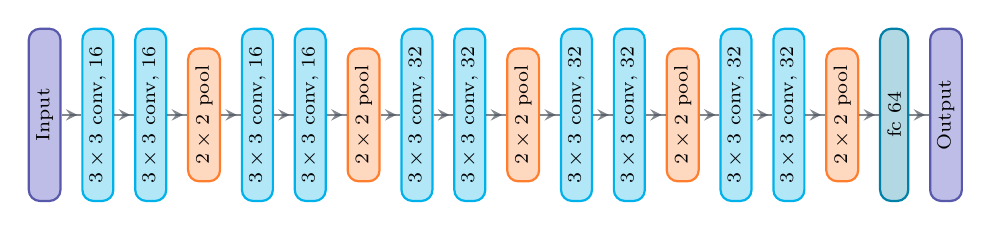
\begin{tikzpicture}[node distance=0.25cm, rotate=90, transform shape] 

\tikzstyle{layer}		=[rectangle, rounded corners, thick, text centered]
\tikzstyle{inp}		=[layer, draw=purple1, fill=purple4, text width=2cm]
\tikzstyle{cv}		=[layer, draw=blue1,	fill=blue4, text width=2cm]
\tikzstyle{pl}		=[layer, draw=orange1, fill=orange4,	text width=1.5cm]
\tikzstyle{fc}		=[layer, draw=bluegray1, fill=bluegray4, text width=2cm]
\tikzstyle{connection}	=[thick, draw=gray1, opacity=0.7, decoration={	markings, 
													mark=at position 0.8 with {\arrow{stealth}}},
													postaction={decorate}]
\scriptsize

\node[inp] 				(inp)  at (0,0)	{Input};

\node[cv, below=of inp] 	(c11) 		{$3\times3$ conv, 16};
\node[cv, below=of c11] 	(c12) 		{$3\times3$ conv, 16};
\node[pl,  below=of c12]	(p1) 			{$2\times2$ pool};

\node[cv, below=of p1] 	(c21) 	 	{$3\times3$ conv, 16};
\node[cv, below=of c21] 	(c22) 		{$3\times3$ conv, 16};
\node[pl,  below=of c22]	(p2) 			{$2\times2$ pool};

\node[cv, below=of p2] 	(c31) 	 	{$3\times3$ conv, 32};
\node[cv, below=of c31] 	(c32) 		{$3\times3$ conv, 32};
\node[pl,  below=of c32]	(p3) 			{$2\times2$ pool};

\node[cv, below=of p3] 	(c41) 	 	{$3\times3$ conv, 32};
\node[cv, below=of c41] 	(c42) 		{$3\times3$ conv, 32};
\node[pl,  below=of c42]	(p4) 			{$2\times2$ pool};

\node[cv, below=of p4] 	(c51) 	 	{$3\times3$ conv, 32};
\node[cv, below=of c51] 	(c52) 		{$3\times3$ conv, 32};
\node[pl,  below=of c52]	(p5) 			{$2\times2$ pool};

\node[fc, below=of p5] 	(fc1) 	 		{fc 64};

\node[inp, below=of fc1] 	(output) 		{Output};

\draw [connection]  (inp.south) -- (c11.north);
\draw [connection]  (c11.south) -- (c12.north);
\draw [connection]  (c12.south) -- (p1.north);

\draw [connection]  (p1.south)   -- (c21.north);
\draw [connection]  (c21.south) -- (c22.north);
\draw [connection]  (c22.south) -- (p2.north);

\draw [connection]  (p2.south)   -- (c31.north);
\draw [connection]  (c31.south) -- (c32.north);
\draw [connection]  (c32.south) -- (p3.north);

\draw [connection]  (p3.south)   -- (c41.north);
\draw [connection]  (c41.south) -- (c42.north);
\draw [connection]  (c42.south) -- (p4.north);

\draw [connection]  (p4.south)   -- (c51.north);
\draw [connection]  (c51.south) -- (c52.north);
\draw [connection]  (c52.south) -- (p5.north);

\draw [connection]  (p5.south)   -- (fc1.north);
\draw [connection]  (fc1.south) -- (output);

\end{tikzpicture}
%%%%%%%%%%%%%%

\end{document}